% Section 8: Conclusions

\section{Conclusions}

Early in the design history of LSST DM datamanagement, we developed a
timeline budget, illustrated in fig. \ref{fig:timeline}, for the major
data handling and processing steps necessary to deliver alerts within
the 60-second required window.  It is worthwhile discerning how our
DC3a results stack up against this budget.  There are three durations
that that are relevant to processing:  image processing/detection
(times 2, for each exposure), association, and alert generation.
Only the first two are part of the DC3a prototype.  

\begin{figure}[t]
\begin{center}
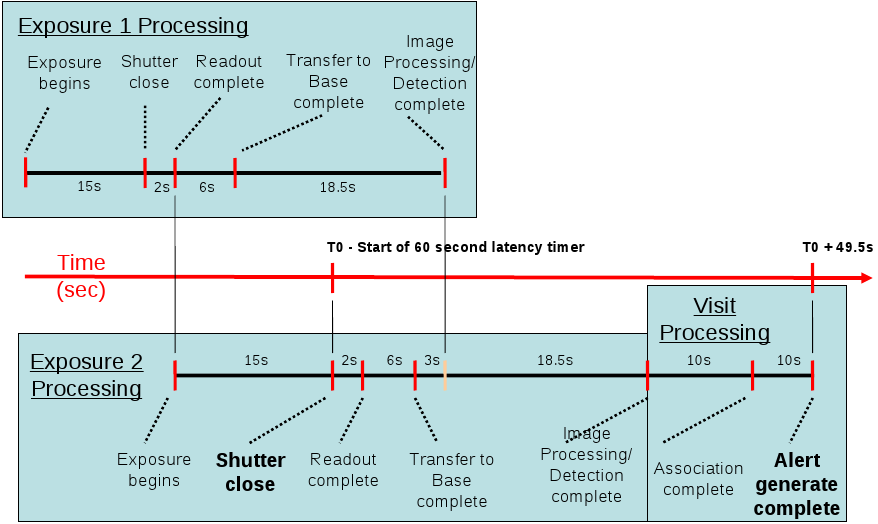
\includegraphics[width=\textwidth]{images/timeline.png}
\caption{A schematic of the alert production time budget.
\label{fig:timeline}}
\end{center}
\end{figure}

Table \ref{tbl:budget} compares the DC3a results with the two
durations in our budget of interest.  We note that, in detail, the
breakdown of our DC3a stages do not neatly map into these duration
categories; for example, there are stages that are done for first
exposure but not the second, and vice version.  In particular, some of
the results from the first exposure is reused for the second.
Nevertheless, a useful rough comparison can be illustrated if we
combine the image processing budgets for each exposure and then take
all production stages (as tagged in table \ref{tbl:ipsdstages},
\Sec{sec:recsummary}) up to and including image subtraction (plus the
time to write out the subtracted image) to constitute image
processing.  (In addition, we will leave out reading in calibration
data assuming this can be done once for the night.)  For association,
we take the remaining stages in IPSD that operate on both exposures
{\it plus} the production stages from AP.  The table breaks the costs
in time between applying science algorithms and I/O (plus the
miscellaneous book-keeping stages).

\begin{table}[htbp]
\centering
\caption{A Comparison of the Alert Production time budget with average
  DC3a costs 
\label{tbl:budget}}
\vspace{\baselineskip}
\begin{tabular}{lc|ccc}
\hline\hline
                           &        & \multicolumn{3}{c}{DC3a Costs}   \\
Budget Category            & Budget & Science    & I/O       & Total   \\
\hline
Image Processing/Detection & 18.5 s & 169.1 s    & 48.3 s    &  s \\
Association                & 10.0 s &   8.7 s    &  2.8 s    &  11.5 s \\
\hline
\end{tabular}
\end{table}

Clearly, we need to improve the performance of the image processing
part by a factor of ten.  We can understand this challenge better by
comparing these totals with the per-stage costs presented in the
Results section; that is, note:

\begin{itemize}
\item Of the 169 seconds spent on science part of image processing, all
  but 6 seconds are spent on image subtraction.
\item 56\% of the I/O time in support of image processing was spent on
  reading in the template sub-images. 
\item Of the 9 seconds spent on the science part of association, all
  but 2 seconds are spent on ``add-and-detect''.  
\end{itemize}

These results, therefore, suggest that the best strategy for meeting
our time budget must include the following:

\begin{itemize}
\item We must substantially improve the image subtraction algorithm.
  As mentioned previously, we believe that 25\% improvement can come
  simply from tuning configuration parameters.  
\item We must develop better strategies for efficient I/O.  In
  particular, significant gains would be gotten via a more
  embarrassingly parallel I/O access to the template data.
\item The decent gains might also be gotten in improvements to the
  add-and-detect stage.  
\end{itemize}



We draw the following conclusions from the results of Data Challenge 3a.

\begin{itemize}
\item Production runs show improvements in DC3a in execution time for common
stages of the IPSD pipeline when compared to DC2. Additional improvement of
execution time is not scoped for DC3b, but will be a major priority for DC4. We
cannot assume that Moore's Law will solve the performance problem for us. We
continue to believe that the processing times necessary for full production
throughput during real-time operation will be reached, but recognize that this
will require considerable attention in DC4.

\item Source detection now is hampered by the quality of the image subtractions.
Registration errors between the calibrated exposure images and the corresponding
template need to be improved; currently misalignment leads to artifacts which
result in many false source detections, along with very strong spurious peaks in
the resulting lightcurves. DC3b will include improvement of the science data
quality as a major focus.

\item Tests on the Abe cluster showed that the pipelines scaled reasonably 
well when applied to the entire focal plane of a CFHT-LS exposure. The 
pipeline stage harness supporting the science algorithms was designed to
be computationally lightweight, and analysis of runs on Abe show that 
comparatively little processing time is spent by this infrastructure.

\item Early in DC3, the code tree underwent significant refactoring and was
additionally upgraded for 64-bit support. These steps were important and
necessary, but left developers without the ability to test implementations
inside the harness framework until comparatively late in the DC3a development
cycle. DC3b will use several strategies, including continuous integration
and additional tools for running science stages independently from the 
LSST cluster.

\end{itemize}
